\section{Contributions}

The primary contributions are obviously the design and implementation of
algorithms for the vision and control logics of the \emph{sense-plan-act} loop,
as well as generating a tailored dataset, but those were not the only tasks to
be done during this research.\\

In the early stages, the use of the Gazebo robotics simulation software was
considered for training a more sophisticated control algorithm later on.
Therefore, the Intel Aero UAV was modeled specifically for this software,
since no other was available. A 3D model was made using the open-source
modeling and rendering software Blender, using the frame model provided by
Intel, and taking dimensions on the physical drone. The Gazebo model is mostly
an integration of several meshes, as well as plugins for each sensor, configured
to match the specifications.

\begin{figure}[h]
	\centering
	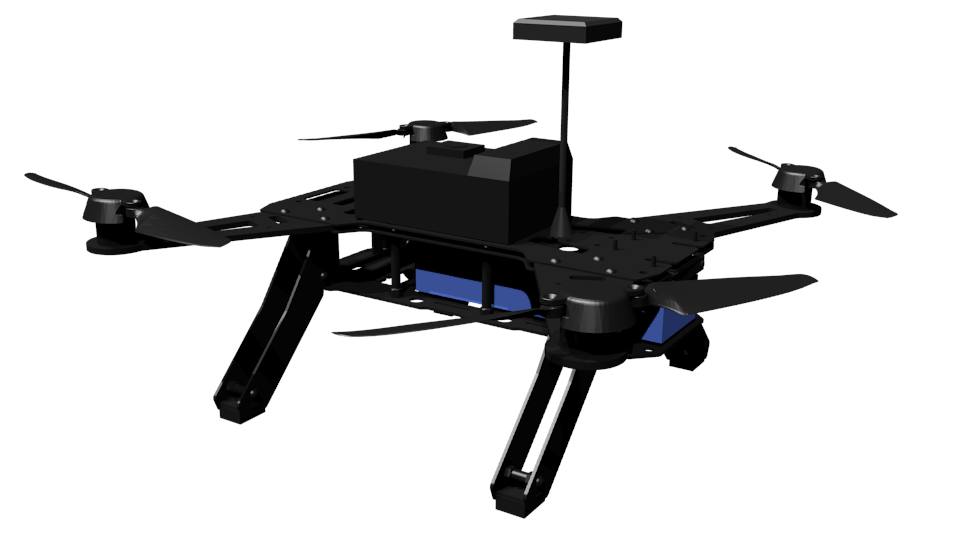
\includegraphics[width=0.5\textwidth]{figure/aero.png}
	\caption{The Intel Aero 3D model made with Blender.}
	\label{fig:aero}
\end{figure}

Furthermore, iterative testing from datasets taken in the AiR Lab showed that
the original gray color of the gates would be too challenging to train a CNN to
detect them, since they were blending in the background because of the motion
blur and noise of the embedded camera. To eliminate this issue, the gates were
painted in four different colors, and one was left unchanged to see if the gate
detection neural network would be robust enough.\\

Lastly, the original propeller guard model, kindly provided by Intel, was
modified for a more solid and convenient 3D printing. Having such protection was
necessary to conduct real flight testing while minimizing the risk of breaking
propellers.
